% !TeX spellcheck = en_US
\documentclass[a4paper,12pt]{article}

\usepackage{fullpage}
\usepackage[utf8]{inputenc}
\usepackage{fourier}
\usepackage{amsmath}
\usepackage{color}
\usepackage{graphicx}
\usepackage{titlesec}
\usepackage{longtable}

\titleformat{\section}[hang]{\Large\bfseries}{\Roman{section}\quad}{0pt}{}
\titleformat{\subsection}[hang]{\large\bfseries}{\arabic{subsection}.\quad}{0pt}{}
\titleformat{\subsubsection}[hang]{\large}{\arabic{subsection}\alph{subsubsection})\quad}{0pt}{}

\newcommand{\twodo}[1]{\textcolor{red}{\textbf{todo:} #1}}

\title{\textbf{Exercises for Image Processing 1}\\Problem Sheet 5}
\author{Tim Dobert\\6427948 \and Konstantin M\"ollers\\6313136}

\begin{document}
	\maketitle	
	
	\section{Theoretical Problems}
	\subsection{(Lossless) Image Compression}
	
	\subsubsection{Entropy}
	
	We calculate the entropy of the document by obtaining the mean number of bits which are required to encode the information of this source. Therefor, we are determine the mean value of all expectable number of bits needed to encode each value. The mean of a value array is calculated by a weighted sum of those values; with the probability being the weight.
	
	\begin{align*}
	\text{Num. of values }G	&= 6 \\
	\text{Entropy } H 	&= \sum\limits_{g = 0}^{G - 1} P(g) \cdot \log_2 \frac{1}{P(g)} 	\\
		&\approx 0.136803+ 0.291508+ 0.0382193+ 0.00996578+ 0.0179316+ 0.0765699\\
		&= 0.570998
	\end{align*}
	
	\subsubsection{Huffman Code}
	
	First of all, we calculate the actual probabilities for the classification in combination with their colors. Because of the independence of these values, we can obtain those just by multiplication.
	
	\begin{table}[h!]
		\centering
		\begin{tabular}{l|l|l|r|l|r}
			$g$ & \textbf{Classification} & \textbf{Color} & \textbf{Probability} $P(g)$ & \textbf{Huffman Code} & \textbf{Length} $l(g)$ \\\hline
			0 & background & white & 0.900 & \texttt{0} & 1 \\
			1 & print & black & 0.080 & \texttt{10} & 2 \\
			2 & print & red & 0.005 & \texttt{1110} & 4\\
			3 & print & yellow & 0.001 & \texttt{11111} & 5\\
			4 & print & green & 0.002 & \texttt{11110} & 5\\
			5 & print & blue & 0.012 & \texttt{110} & 3\\\hline
			\multicolumn{3}{l|}{$\Sigma$} & 1.000 & \multicolumn{2}{r}{1.131}
		\end{tabular}
	\end{table}
	
	The Huffman code gets calculated by giving the smallest probabilities a binary code (either \texttt{0} or \texttt{1}) and summing up their probabilities. We then compare the sum with other values and iterate. In the end, you get a code The way we calculated the Huffman code is presented in the following schema.
	
	\begin{figure}[h!]
		\centering
		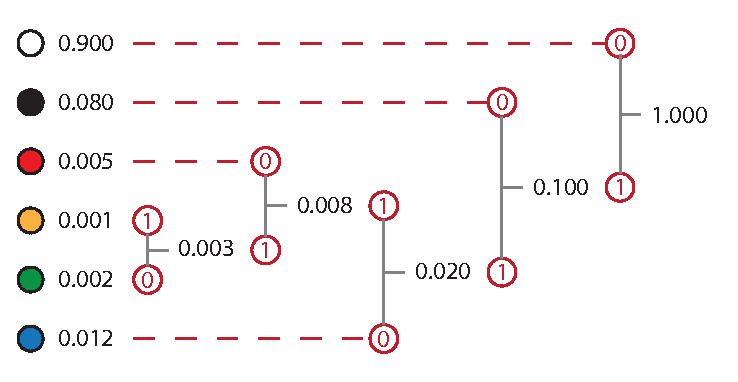
\includegraphics[width=0.7\textwidth]{huffman.pdf}
	\end{figure}
	
	\newpage
	
	\subsubsection{Mean Length}
	
	To calculate the mean length $b_\text{Huffman}$ of our Huffman code, we just need to sum up the probability-weighted code lengths of all pixel values.
	
	\begin{align*}
		b_\text{Huffman} &= \sum\limits_{g = 0}^{G - 1} P(g) \cdot l(g)\\
			&= 0.900 \cdot 1\\
			&+ 0.080 \cdot 2\\
			&+ 0.005 \cdot 4\\
			&+ 0.001 \cdot 5\\
			&+ 0.002 \cdot 5\\
			&+ 0.012 \cdot 3 = 1.131
	\end{align*}
	
	{\footnotesize Redundancy $r_\text{Huffman} = 1.131 - 0.570998 = 0.560002$.}
	
	\subsubsection{Redundancy}
	
	{\footnotesize With formulas from Lecture 08, Slide 5:}
	\begin{align*}
		\text{Num. bits per pixel }b_\text{4-bit} &= 4 \\
		\text{Entropy }H &\approx 0.570998\\
		\text{Redundancy }r_\text{4-bit} &= b_\text{4-bit} - H \approx 3.429002
	\end{align*}
	
	
	\noindent As we can see, our Huffman code is much less redundant than the 4-bit code given from the exercise; as the latter has a redundancy value of 3.429002 whether the former has just one of 0.560002.
	
	\subsection{Image Segmentation}

	\section{Practical Problems}
	\subsection{(Lossy) Image Compression}
	\subsection{Operators for Edge detection}
	
	This how the angles are colored in the following direction images: \quad
	\raisebox{-1.9cm}{\includegraphics[width=4cm]{kompass}}
	
	\begin{longtable}{@{}p{\dimexpr\textwidth-8.5cm}@{}p{4cm}@{\hspace{.5cm}}p{4cm}@{}}
		& \raisebox{-\totalheight}{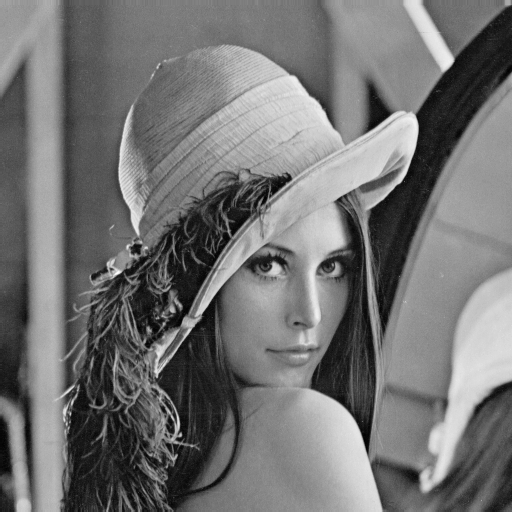
\includegraphics[width=\linewidth]{lena}} \linebreak \textit{Original Image}&\\
%		
		a) \textbf{Robert's Cross operator} \par
		Looks very noisy
		& \raisebox{-\totalheight}{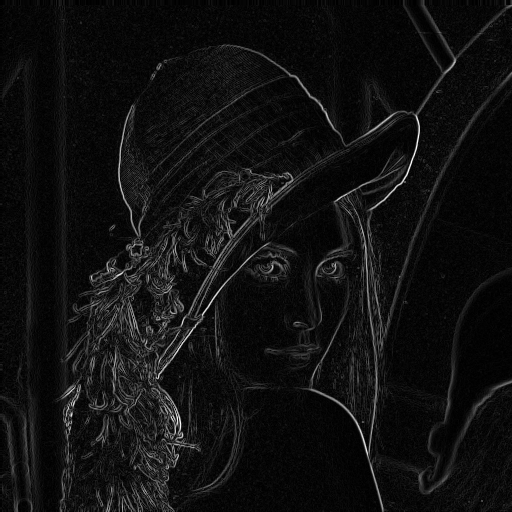
\includegraphics[width=\linewidth]{roberts_cross_magnitudes}} \linebreak \textit{Magnitudes}
		& \raisebox{-\totalheight}{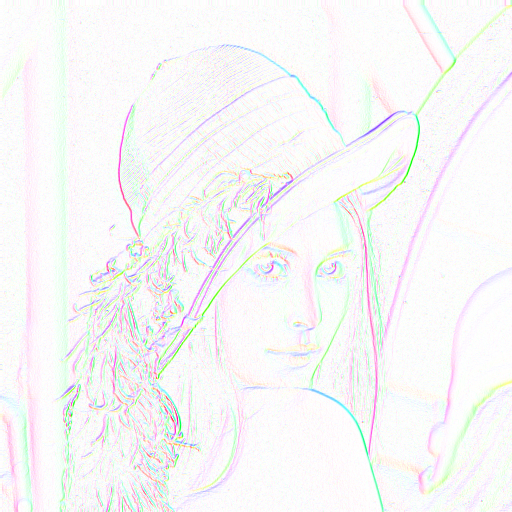
\includegraphics[width=\linewidth]{roberts_cross_directions}} \linebreak[1cm] \textit{Directions}\\
%		
		b) \textbf{Sobel operator} \par
		& \raisebox{-\totalheight}{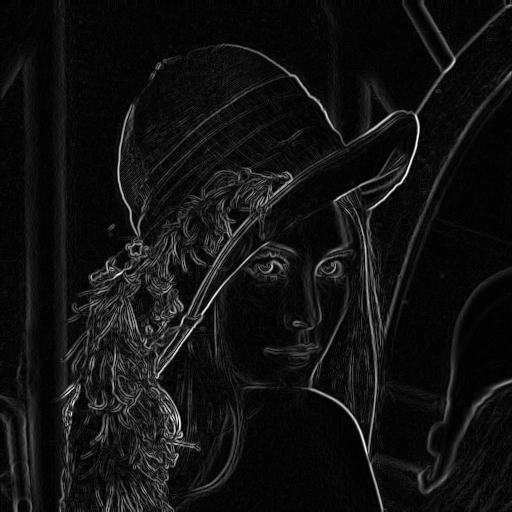
\includegraphics[width=\linewidth]{sobel_magnitudes}} \linebreak \textit{Magnitudes}
		& \raisebox{-\totalheight}{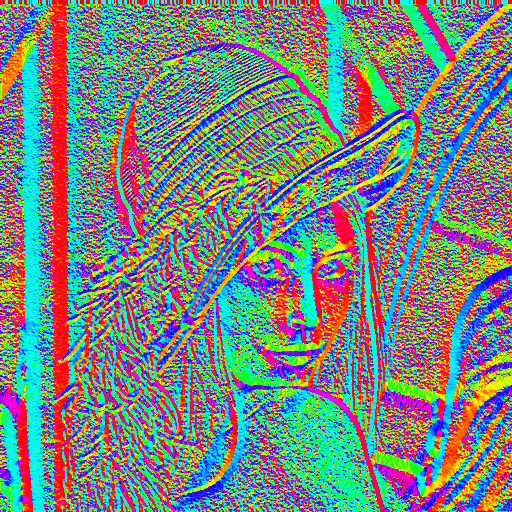
\includegraphics[width=\linewidth]{sobel_directions}} \linebreak \textit{Directions}\\
%		
		c) \textbf{Kirsch operator}  \par
		& \raisebox{-\totalheight}{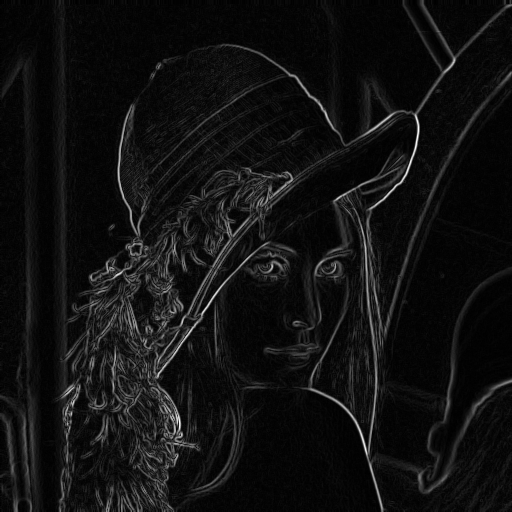
\includegraphics[width=\linewidth]{kirsch_magnitudes}} \linebreak \textit{Magnitudes}
		& \raisebox{-\totalheight}{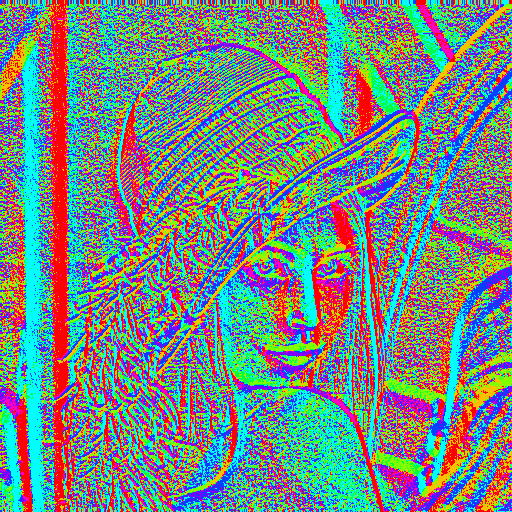
\includegraphics[width=\linewidth]{kirsch_directions}} \linebreak \textit{Directions}\\
%		
		d) \textbf{Laplacian operator} \par
		& \raisebox{-\totalheight}{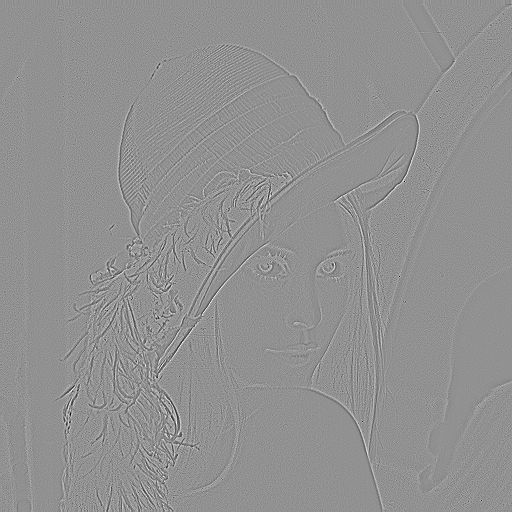
\includegraphics[width=\linewidth]{laplacian}} \linebreak \textit{2\raisebox{2pt}{\footnotesize nd} Derivative}
		&
	\end{longtable}
	
	We would prefer the \textbf{Sobel operator}, because with it it's the easiest to recognize details of the face like eyes, lips and nose.

\end{document}
